% MIRAR VIDEO

%%%%%%%%%%%%%%%%%%%%%%%%%%%%%%%%%%%%%%%%%%%%%%%%%%%%%%%%%%%%%%%%%%%%%%%%%%%%%%%%%

\clearpage
\section{Schemes and plots}
\noindent First, let's derive the output of both systems so as to be able to easily solve the $4$ questions that appear on the next section.

\begin{figure}[H]
   \centering
   \begin{circuitikz}[>=latex'][american]
   \tikzstyle{block} = [draw, rectangle, minimum height=1cm, minimum width=2cm]
   \draw (2.5,-2.5) node[oscillator, scale=1.19] (mixer1) {};
   \draw (2.5,-0.5) node[oscillator, scale=1.19] (mixer2) {};
   \draw (3.0,-0.5) node[] {$i(t)$};
\draw (3.95,-2.5) node[] {$V(t) = V_0 \cos(w_0 t)$};
   \draw (5.0,1.5) node[block, scale=1] (block1) {$\frac{1}{T} \int_0^T x(t) dt$};
   \draw (5.0,4.0) node[block, scale=1] (block2) {LPF};
   \draw (2.0,-4.5) node[ground]{};
   \draw (2.0,-3.0) to[short] (2.0,-4.5);
   \draw (2.0,-1.0) to[short] (2.0,-2.0);
   \draw (2.0,-0.0) to[short] (2.0,1.5);
   \draw (2.0,1.5) to[short] (4.0,1.5);
   \draw (6.0,1.5) to[short] (7.5,1.5);
   \draw (2.0,1.5) to[short] (2.0,4.0);
   \draw (2.0,4.0) to[short] (4.0,4.0);
   \draw (6.0,4.0) to[short] (7.5,4.0);
   \end{circuitikz}
   \caption{Schematic of the exercise}
\end{figure}

\noindent Where the integrator performs
\begin{equation}
   y(n) = \frac{1}{T} \int_{0}^T x(t) dt \ .
\end{equation}
\noindent Where $T$ is the integration time. When the input to this block is $V(t) = V_0 \cos(w_0 t + \phi) = V_0 \sin(w_0 t + \phi_2)$, where $\phi_2 = \frac{\pi}{2} + \phi$, we have 
\begin{equation}
   y(n) = \frac{1}{T} \int_0^T V_0 \sin(w_0 t + \phi_2) = V_0 \frac{1}{w_0} \frac{1}{T} \left[ \cos(w_0 T + \phi_2) - \cos(\phi_2) \right] \ .
\end{equation}
\noindent The idea here is to manipulate the expression so that we can express the output in terms of the input and a $\sin()$ or $\cos()$ function. In the slides, the previos equation is rewritten as
\begin{equation} \label{eq:good}
   y(n) = \frac{2}{w_0 T} V_0 \sin(\frac{w_0 T}{2} + \phi_2) \sin\left(\frac{w_0 T}{2}\right) \ .
\end{equation}
\noindent To make sure this is correct, trigonometric functions can be expanded using Euler's identity. We want to prove 
\begin{equation}
   \cos(w_0 T + \phi_2) - \cos(\phi_2) = 2 \sin\left(\frac{w_0 T}{2} + \phi_2 \right) \sin\left(\frac{w_0 T}{2}\right) \ .
\end{equation}
\noindent This previous equation becomes
\begin{equation}
   \begin{split}
      \frac{e^{j \left( w_0 T + \phi_ 2\right)} + e^{- j (w_0 T + \phi_2)}}{2} - \frac{e^{j \phi_2} + e^{-j \phi_2}}{2} &= 2 \frac{e^{j \frac{w_0 T}{2}} - e^{-j \frac{w_0 T}{2}}}{2} \frac{e^{j \left( \frac{w_0 T}{2} + \phi_2 \right)} - e^{-j \left( \frac{w_0 T}{2} + \phi_2 \right)}}{2} \\
      e^{j \left(w_0 T + \phi_ 2\right)} + e^{-j (w_0 T + \phi_2)} - e^{j \phi_2} + e^{- j \phi_2} &= \left( e^{j \frac{w_0 T }{2}} - e^{-j \frac{w_0 T }{2}} \right) \left( e^{j \left(\frac{w_0 T}{2} + \phi_2 \right)} - e^{-j \left(\frac{w_0 T}{2} + \phi_2 \right)} \right) \\
      e^{j (w_0 T + \phi_2)} + e^{-j (w_0 T + \phi_2)} - e^{j \phi_2} + e^{-j \phi_2} &= e^{j (w_0 T + \phi_2)} + e^{-j (w_0 T + \phi_2)} - e^{j \phi_2} + e^{-j \phi_2}
   \end{split} \ .
\end{equation}
\noindent So, yes, \eqref{eq:good} is correct. Now, $\sin()$ is transformed back to $\cos()$.
\begin{equation} \label{eq:good}
   y(n) = \frac{2}{w_0 T} V_0 \cos(\frac{w_0 T}{2} + \phi) \sin\left(\frac{w_0 T}{2}\right) \ .
\end{equation}
\noindent This is the output out of the integrator. It can also be written as
\begin{equation}
   y(n) = \frac{1}{\pi f T} V_0 \cos(\pi f T + \phi) \sin\left( \pi f T \right) = V_0 \cos(\pi f T + \phi) \frac{\sin(\pi f T)}{\pi f T} \ .
\end{equation}
\noindent Where $f$ is the frequency of $w_0$, i.e., the frequency of the signal. The $\frac{\sin(\pi f T)}{\pi f T}$ is the sinc function, so it can output values of up to $1$, and $0$ when $fT$ is an integer number.

\noindent One can wonder what's the output of the LPF. In this case, we have to keep in mind this system shows the same bandwidth as for the discrete integrator. Then, the output of this system must be tangent to the output of the discrete integrator only in the points in which the discrete integrator output is maximum. There's a plot about SMRR on the slides that can be of help in visualizing this.

\noindent I plot the derived expression and the expression of the other system, without multiplying them by the input signal. The module is taken. % $V_0 \cos(\pi f T + \phi)$.
\begin{figure} [H] \centering  
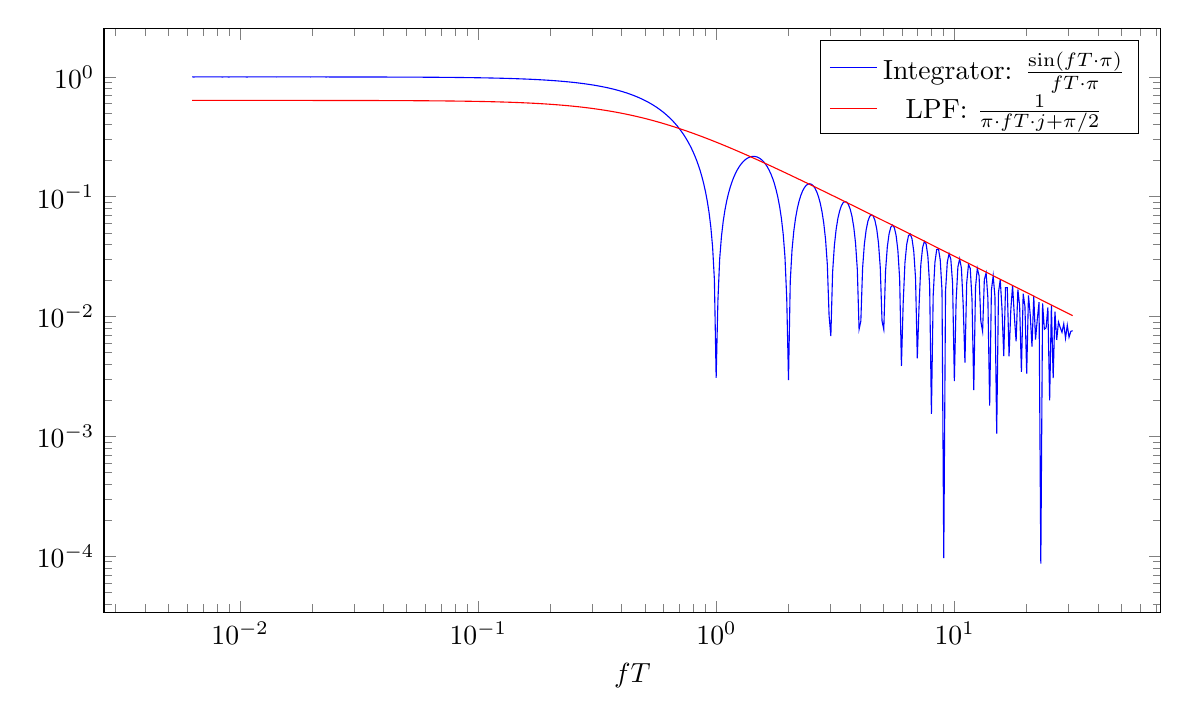
\begin{tikzpicture}
   \begin{axis}[
           % xmin=0, xmax=1, % x scale
           % ymin=0, ymax=1, % y scale
           % ymax = 1.5, ymin = -1.5,
	   	   width=15cm, height=9cm,
           domain = 0.001*2*pi:5*2*pi, samples = 500,
           xmode = log, ymode=log,
           xlabel={$f T$},
   ]
   % \addplot [blue,no marks]    { abs( 1*cos(deg(x)/pi)*sin(deg(x))/ (x) )  };
   % \addplot [red,no marks]    { abs( 1*cos(deg(x)/pi)/x ) };

  %  \addplot [blue,no marks]    { abs( 1*cos(deg(x*pi))*sin(deg(x*pi))/ (x*pi) )  };
   % \addplot [red,no marks]    { abs( 1*cos(deg(x*pi))/(x*pi) ) };
   % \legend{$\cos(x) \frac{\sin(x)}{x}$, $\cos(x) \frac{1}{x}$};
   \addplot [blue,no marks]    { abs( 1*sin(deg(x*pi))/ (x*pi) )  };
   %\addplot [red,no marks]    { abs( 1/(x*pi) ) };
   \addplot [red,no marks]    { abs( 1/(sqrt((pi/2)^2 + (3.14*x)^2)) ) };
   %\legend{$ \frac{\sin(x \cdot \pi)}{x \cdot \pi}$, $ \frac{1}{x\cdot \pi}$};
   \legend{Integrator: $ \frac{\sin(f T \cdot \pi)}{f T \cdot \pi}$, LPF: $ \frac{1}{\pi \cdot f T \cdot j + \pi/2}$};

   % \addplot [red,mark=square*] coordinates{(.125, .744)};
   \end{axis}
\end{tikzpicture}
\caption{Output of the 2 integrators}
\end{figure}
%
\noindent The LPF equation has been derived the following way. Initially, I wrote the following generic low pass filter equation:
\begin{equation}
   LPF = \frac{k}{b \cdot f T j + a} \ .
\end{equation}
\noindent Where $k$, $b$, and $a$ are constants to determine, and $j = \sqrt{-1}$. First, I wanted to be compliant with the specified bandwidth $BW = \frac{1}{2 T}$. Second, I wanted the same slope for high frequencies. Thus,
\begin{equation}
   \begin{split}
      \frac{k}{b} &= \frac{1}{\pi} \\
      f_{-3 dB} &= \frac{1}{2 T} \\
      f_{-3 dB} &= \frac{a}{b T} \\
   \end{split} \ .
\end{equation}
\noindent With this, and setting $k=1$, I get
\begin{equation}
   \begin{split}
      b &= \pi \\
      a &= \frac{\pi}{2}
   \end{split} \ .
\end{equation}
\noindent Leading to 
\begin{equation}
   LPF = \frac{1}{\pi f T j + \frac{\pi}{2}} \ .
\end{equation}
\noindent Notice that this is the exact eequation that has been plotted above, and that for $-3$ dB both plots intersect, meaning they have the same bandwidth. The bandwidth $BW = \frac{1}{2 T}$ was a specification given in the statement. As it has been proven, it's the correct value to have the two bandwidths to be equal.


% First, I noticed I want a gain of $1$ in linear units in the flat region, so that for low frequencies I get at the output the exact same signal I had at the input. Then, for high frequencies, I want to get the envelope of the sinc() function, i.e., $\frac{1}{fT \cdot \pi}$.

\noindent So, what's the output of the LPF for a sinusoidal input $V(t) = V_0 \cos(w_0 t + \phi) =  V_0 \cos(2 \pi f t + \phi)$? Well, taking into account the gain and the phase of the system,
\begin{equation}
   y = V_0 \frac{1}{\sqrt{ \left(\frac{1}{4} \right)^2 + (\pi f T)^2}} \cos \left(  2 \pi f t + \phi - \arctan \left( 4 \pi f T \right) \right) \ .
\end{equation}

% Notice the -3 dB point is not equal for the two systems...


% \noindent To gain more insight, I derive the output of the low pass filter. One possibility is to define it as $H(s) = \frac{1}{s}$. If $V_n \cos(w t)$ is the input to the system, the output $Y(s)$ will be
% \begin{equation}
   % Y(s) = \frac{K}{s} V_n \frac{s}{s^2 + w^2} = V_n K \frac{1}{w} \frac{w}{s^2 + w^2} \ .
% \end{equation}
% \noindent This can be anti-transformed to get the temporal output
% \begin{equation}
   % y(t) = V_n \frac{K}{w} \sin(w t) = V_n \sin(2 \pi f t) \frac{K}{2 \pi f} \ .
% \end{equation}
% \noindent Now, the question is what's the value of $K$? Setting the factor that multiplies the input of the discrete integrator output to $-3$ dB we will be able to calculate $\pi f T$, by equating the bandwidth of the $2$ systems.
% \begin{equation}
   % \frac{\sin(\pi f T)}{\pi f T} = \frac{1}{\sqrt{2}}  \ .
% \end{equation}
% \noindent This leads to 
% \begin{equation}
   % \pi f T |_{-3dB} = 1.39156 \ .
% \end{equation}
% \noindent Now, we set the output of the LPF to $\frac{1}{\sqrt{2}}$ and consider $\sin(2 \pi f t) = 1$. This leads to
% \begin{equation}
   % \begin{split}
         % \frac{K}{2 \pi f|_{-3dB}} =& \frac{1}{\sqrt{2}} \\
         % \frac{K}{2 \pi \frac{1.39156}{\pi T}} =& \frac{1}{\sqrt{2}} \\
   % \end{split}
% \end{equation}
% \noindent With this,
% \begin{equation}
   % \begin{split}
      % K &= \frac{2}{\sqrt{2}} \frac{1.39156}{T} \\
      % K &= \frac{1.96796}{T} \approx \frac{2}{T}
   % \end{split} \ .
% \end{equation}
% \noindent Going back to the output of the LPF, notice that now
% \begin{equation}
   % y(t) = V_n \frac{K}{w} \sin(w t) = V_n \sin(2 \pi f t) \frac{\frac{2}{T}}{2 \pi f} \ .
% \end{equation}
% \noindent So,
% \begin{equation}
   % y(t) = V_n \sin(2 \pi f t) \frac{1}{\pi f T} \ .
% \end{equation}




% \noindent Thanks to the previous reasoning, it can be said that the output of the LPF system, for a sinusoidal input $V_0 \cos(\pi f T)$ will be
% \begin{equation}
   % y(t) =  V_0 \sin(2 \pi f t + \phi) \frac{1}{\pi f T} \ .
% \end{equation}
% \noindent In essence, the LPF integrates the input signal, so if the input is a cosine function, the output is a sine function. Moreover, one must notice the term $\frac{1}{2 \pi T}$. This is compliant with having the same bandwidth for both systems, as imposed in the previous development. We obtain the factor that is plotted in red in the previos plot, which acts as a limit to the discrete integrator output.

\noindent Now, we know how will be the output of both systems when a cosine with a certain frequency and amplitude is applied. We are in a position to solve the next questions. If $w \geq 0$, we will just have to plug this into the outputs of the two systems. If there's a signal but also an interference, we can apply the superposition theorem.


\section{Exercise 3}
\begin{pexbox}{}
    \textbf{a) For $i(t) = 0$ and $w_0 = 0$ demonstrate that the amount information out of both systems is the same.}
\end{pexbox}

\noindent In this case, there's no interference. It's enough to evaluate the output of both systems for the same applied input signal, $V(t) = V_0 \cos(w_0 t)$. We have already analyzed the output of both systems for a signal like this.
\begin{equation}
   \begin{split}
   y_1 &=  V_0 \cos(\pi f T + \phi) \frac{\sin(\pi f T)}{\pi f T} \\
   % y_2 &=  V_0 \sin(2 \pi f t + \phi) \frac{1}{\pi f T} 
   y_2 &= V_0 \frac{1}{\sqrt{ \left(\frac{1}{4} \right)^2 + (\pi f T)^2}} \cos \left(  2 \pi f t + \phi - \arctan \left( 4 \pi f T \right) \right) 
   \end{split} \ .
\end{equation}
\noindent In this case, $\phi = 0$. Now, we can perform the calculations for $f \rightarrow 0$. The identity $\frac{\sin(x)}{x}|_{x \rightarrow 0} \approx \frac{x}{x} \approx 1$ can be of help. Then,
\begin{equation}
   \begin{split}
   y_1|_{f\rightarrow 0} &=  V_0 \cos(\pi f T + \phi) \frac{\sin(\pi f T)}{\pi f T} \approx V_0 \\
   % y_2|_{f\rightarrow 0} &=  V_0 \sin(\pi f t + \phi) \frac{1}{\pi f T} \approx V_0 (\pi f t + \phi) \frac{1}{\pi f T} = V_0 \frac{t}{T} % \infty
   y_2|_{f\rightarrow 0} &=  V_0 \frac{1}{\sqrt{ \left(\frac{1}{4} \right)^2 + (\pi f T)^2}} \cos \left(  2 \pi f t + \phi - \arctan \left( 4 \pi f T \right) \right) = 4 V_0 % \infty
   \end{split} \ .
\end{equation}
\noindent Recall $\phi = 0$. The output of the integrator could already be deduced from the above plot without problems. While it's harder to appreciate on the plot the output of the LPF for this case, it's easy to verify that it must be equal to $4 V_0$. The LPF equation can be analyzed for $f\rightarrow 0$ and the $4$ factor arises. %  while the output of the LPF shows the $\frac{1}{T}$ factor, which means that for low values of $T$ the output is going to be large. Also, it's worth noticing that at both outputs the interference, or the noise, will be $N=0$. The information formula is

\noindent What's important to realise is that at both outputs the interference, or the noise, will be $N=0$. The information formula is
\begin{equation}
   I = B \log_2 \left( 1 + \frac{S}{N} \right) \approx 3.32 B \log_{10} \left( 1 + \frac{S}{N}\right) \ .
\end{equation}
\noindent As both noises are $0$, % and assuming $t>0$,
\begin{equation}
   \boxed{
      I_1 = I_2 = \infty
   } 
\end{equation}
\noindent Keep in mind this is a theoretical limit. In practice, this will never be achieved.



\begin{pexbox}{}
    \textbf{b) For $i(t) = 0$ and $w_0 > 0$ demonstrate that the amount information out of both systems is the same. Are there any restrictions on the relationship $T$ and $w_0$?}
\end{pexbox}

\noindent Going back to the equations, notice that for $f>0$ the output formulas we obtained previously should be analyzed carefully: % can no longer be $\infty$, in any case.
\begin{equation}
   \begin{split}
   y_1 &=  V_0 \cos(\pi f T + \phi) \frac{\sin(\pi f T)}{\pi f T} \\
   % y_2 &=  V_0 \sin(\pi f t + \phi) \frac{1}{\pi f T} 
   y_2 &=  V_0 \cos \left(  2 \pi f t + \phi - \arctan \left( 4 \pi f T \right) \right) \frac{1}{\sqrt{ \left(\frac{1}{4} \right)^2 + (\pi f T)^2}} 
   \end{split} \ .
\end{equation}
\noindent As long as $f T \not\subset \mathbb{Z} $, i.e., the $fT$ factor is not an integer, then $\sin(\pi f T) \neq 0$, so there's a signal out of the first system.

\noindent For the second system, the LPF, for certain instants of time $t$ there's the risk to get a $0$ output. However, what's of interest here is to notice the output signal will attenuated a certain amount, as the plot suggestes. Of course, for the integrator, if we had integrated from $t_1$ to $t_2$ instead of from $0$ to $T$, we would also depend on these values of time to assure wether the output is zero or not. The key idea is to not be bothered about the value the input signal takes at the input, but to get an idea about the relation between input and output (gain). For this, the plot can be of great help.  % both systems. Given that there's no noise, both informations will be $\infty$, again.

\noindent Given that there's no noise, it's direct to see that
\begin{equation}
   \boxed{
      I_1 = I_2 = \infty
   } 
\end{equation}
\noindent Recall this is only true if
\begin{equation}
   \boxed{
      \frac{w_0}{2 \pi} T \not\subset \mathbb{Z}
   }
\end{equation}
\noindent This condition guarantees that we don't integrate over a whole number of periods, as for this case the integral would be $0$. This is a very important condition that could be derived for the plot. 

\noindent On the other hand, if it happens that the $\cos()$ of $y_2$ is $0$ for a certain instant of time, we shouldn't bother much, as for other instants of time we will get a signal. For the LPF the signal suffers attenuation and phase shift, but in any case it's gain goes to $0$, i.e., attenuation goes to $\infty$. This is a key concept that can be useful for d) section.



\begin{pexbox}{}
    \textbf{c) For $i(t) = n (t)$, $w_0 > 0$ and the above restrictions, demonstrate that the amount information out of both systems is the same.}
\end{pexbox}

\noindent So now, thanks to "the above restrictions", we can assume the frequency and the period of integration product don't result in an integer number. 

\noindent Notice that now we have white Gaussian noise, which means that in the frequency spectrum we have a constant PSD from $-\infty$ to $\infty$, and in the time domain it follows a Gaussian distribution of $0$ mean. It is well known that the integration of this noise must lead to an average value of $0$ \footnote{\href{https://ocw.mit.edu/courses/electrical-engineering-and-computer-science/6-02-introduction-to-eecs-ii-digital-communication-systems-fall-2012/readings/MIT6_02F12_chap09.pdf}{MIT notes on noise}.}. Of course, there will be some uncertainty in this $N=0$ (noise equals $0$) average value, but here we are looking at average values. Then, provided $ \frac{w_0}{2 \pi} T \not\subset \mathbb{Z}$,
\begin{equation}
   \boxed{
      I_1 = I_2 = \infty
   } 
\end{equation}


\begin{pexbox}{}
   \textbf{d) What happens if $i(t) = V_i \cdot \sin(w_i t)$?}
\end{pexbox}

\noindent Now, the interference is no longer white Gaussian noise. We can apply the superposition theorem and the previous expressions to affirm that
%
\begin{equation}
   \begin{split}
   y_1 =&  V_0 \cos(\pi f T + \phi) \frac{\sin(\pi f T)}{\pi f T} +  V_i \cos(\pi f_i T + \phi) \frac{\sin(\pi f_i T)}{\pi f_i T} \\
   y_2 =& V_0 \cos \left(  2 \pi f t + \phi - \arctan \left( 4 \pi f T \right) \right) \frac{1}{\sqrt{ \left(\frac{1}{4} \right)^2 + (\pi f T)^2}} \\ &+ V_i \cos \left(  2 \pi f_i t + \phi - \arctan \left( 4 \pi f_i T \right) \right) \frac{1}{\sqrt{ \left(\frac{1}{4} \right)^2 + (\pi f_i T)^2}}  
   % y_2 &=  V_0 \sin(\pi f t + \phi) \frac{1}{\pi f T}  + V_i \sin(\pi f_i t + \phi) \frac{1}{\pi f_i T}  
   \end{split} \ .
\end{equation}
\noindent Where $f_i$ is the frequency of the interference signal and $V_i$ its amplitude, and $f$ is the frequency of the signal and $V_0$ its amplitude. Each one of the informations is depicted here:
\begin{equation}
   \begin{split}
      % I_1 &= B \log_2 \left(1 + \frac{ V_0 \cos(\pi f T + \phi) \frac{\sin(\pi f T)}{\pi f T} }{V_i \cos(\pi f_i T + \phi) \frac{\sin(\pi f_i T)}{\pi f_i T}}  \right)  = B \log_2 \left(1 + \frac{ V_0 \cos(\pi f T + \phi) \frac{\sin(\pi f T)}{ f } }{V_i \cos(\pi f_i T + \phi) \frac{\sin(\pi f_i T)}{ f_i }}  \right) \\
      % I_2 &= B \log_2 \left(1 + \frac{ V_0 \sin(\pi f t + \phi) \frac{1}{\pi f T}}{ V_i \sin(\pi f_i t + \phi) \frac{1}{\pi f_i T}  } \right) =  B \log_2 \left(1 + \frac{ V_0 \sin(\pi f t + \phi) \frac{1}{ f }}{ V_i \sin(\pi f_i t + \phi) \frac{1}{f_i }  } \right)  \\
      I_1 &= B \log_2 \left(1 + \frac{ V_0 \cos(\pi f T + \phi) \frac{\sin(\pi f T)}{\pi f T} }{V_i \cos(\pi f_i T + \phi) \frac{\sin(\pi f_i T)}{\pi f_i T}}  \right)  \\
      I_2 &= B \log_2 \left(1 + \frac{ \frac{ V_0 \cos \left(  2 \pi f t + \phi - \arctan \left( 4 \pi f T \right) \right)}{\sqrt{ \left(\frac{1}{4} \right)^2 + (\pi f T)^2}} }{ \frac{ V_i \cos \left(  2 \pi f_i t + \phi - \arctan \left( 4 \pi f_i T \right) \right)}{\sqrt{ \left(\frac{1}{4} \right)^2 + (\pi f_i T)^2}} } \right)  \\
   \end{split} \ .
\end{equation}
%
\noindent For $y_1$, i.e., the output out of the discrete integrator, we could set  $f_i T \subset \mathbb{Z} $ so that the interference is totally eliminated. Then, we could still get $I_1=\infty$, theoretically. In reality, noise will never be totally eliminated, though, but we can potentially get a very nice SNR (signal-to-noise ratio).

\noindent For $y_2$, which is the output of the LPF, we can't attenuate the noise. In this case, probably the signal level will be higher than for $y_1$, but there's no way to effectively attenuate only the noise. 

\noindent All in all, if the $T$ value is adjusted so as to eliminate the noise interference, and $f_i$ is known, one can expect a much higher theoretical information bound for $y_1$ than for $y_2$, $I_1 > I_2$. The previous plot shows how this technique can be very effective in improving the signal-to-noise ratio, if $T$ is adjusted correctly, $f_i$ is known, and there's some separation between the interference and the signal frequencies.



% \chapter{Uncertainty evaluation in time measurements}


% \section{Statement}

% \begin{graytext}

   % \noindent \textbf{Estimate the uncertainty in measuring the following magnitude:}

   % \noindent \textbf{-The frequency of a $50$ Hz sinusoidal signal of about $1 \text{ V}_{\text{RMS}}$ with a superimposed white noise of $1 \text{ mV}_{\text{RMS}}$.}
   
   % \noindent \textbf{When using the following instrument: KEYSIGHT 53230A (manufacturer's way AND  GUM way) for two different measurement times: $100$ ms and $10$ s}

   % \noindent \textbf{Critically compare both results.}

   % \noindent \textbf{*Use the best oscillator option available (no external oscillator).}
% \end{graytext}


% \clearpage
% \section{Uncertainty assessment manufacturer's way}
 
% \noindent First, I carry on the calculations using the KEYSIGHT 53230A manufacturer's information that is provided in the datasheet. There's a worked example at the end of the datasheet that can be of help.

% \noindent First, the manufacturer defines the expanded uncertainty $U_e$ (they call it basic accuracy) as
% \begin{equation}
   % U_e = \pm \left[ k \cdot u_{random} + u_{systematic} + u_{timebase} \right] \ .
% \end{equation}
% \noindent Where the $u_{random}$, the Random Uncertainty, is due to input noise at the instrument (either from the signal we want to know the frequency of) or the equipment itself, apart from other factors. Systematic Uncertainty, $u_{systematic}$, is inversely proportional to gate time, as we shall later see. Timebase Uncertainty, $u_{timebase}$, comes from the oscillator. In next sections each one of these uncertainties is defined, so as to perform the calculations later.


% \subsection{Random uncertainty}
% \noindent For $u_{random}$, the manufacturer provides the following formula:
% \begin{equation}
   % u_{random} = \frac{1.4 \sqrt{T_{SS}^2 + T_E^2}}{R_E \cdot GT} \ .
% \end{equation}
% \indent $T_{SS}$: single shot timing.\\
% \indent $T_{E}$: threshold error.\\
% \indent $R_{E}$: Resolution enhancement factor, calculates the added frequency resolution beyond the basic reciprocal measurement capability.\\
% \indent $GT$: Gate time.\\

% \noindent The Gate time is either $10$ s or $100$ ms in this exercise. But what about the other variables? Let's break them down.

% \noindent First, for $T_{SS}$,
% \begin{equation}
   % T_{SS} = 20 \text{ ps} \ .
% \end{equation}
% \noindent We are given this value in page 8 as well as in page 22. This is in fact the timing resolution we have.

% \noindent For $T_E$, the manufacturer provides the following formula for a $\pm 5$ V input range, which is suitable for our signal.
% \begin{equation}\label{eq:TE}
   % T_E = \frac{\sqrt{\left(500 \ \mu\text{Vrms}\right)^2 + E_N^2 + V_X^2}}{\text{ SR at trigger}} \ .
% \end{equation}
% \indent $500 \ \mu$V: comes from page 5, it's the maximum equivalent input noise the 53230A instrument can have at its input port.\\
% \indent $E_N$: input signal noise. We are given $E_N = 1 \text{ mV}_{\text{RMS}}$, so no need to integrate a PSD from $0$ Hz to $350$ MHz.\\
% \indent $V_X$: according to the specifications, $V_X = 0$ when no signal is applied to the other standard input channel, which can be assumed to be our case.\\
% \indent SR at trigger: the slew rate that the input signal has at the trigger point. SR at trigger $= \sqrt{2} \cdot 2 \pi 50$ V/s. It's calculated by applying the derivative to the input signal and taking the slope at a $0$ V cross.

% \noindent From all this, and by noticing that $T_E$ does not depend on the measurement time, we can already calculate its value.
% \begin{equation}
   % T_E = \frac{\sqrt{\left(500 \ \mu\text{Vrms}\right)^2 + (1 \text{ mVrms})^2 + 0^2}}{ \sqrt{2} \cdot 2 \pi 50} = 2.51646 \cdot 10^{-6} \text{ s} \ .
% \end{equation}
% \noindent To me, applying this equation makes a lot of sense. The instrument input noise and the signal noise are assumed to be uncorrelated. Then, the way to sum them is to square them, sum them, and calculate the square root. But notice the units of this result is V, while we are interested in a time magnitude. Well, assuming the threshold is at $0$ V and our input signal has no offset, we can know the slope of the voltage over time at this point. This magnitude allows us to transform from voltage to time, and so we get a time uncertainty. This exact same calculation is performed later for the GUM method.

% %
% \noindent Next, the resolution enhancement factor $R_E$ should be known. According to the manufacturer, $R_E \geq 1$ always applies. To be more concrete, the manufacturer says:
% \begin{equation}
   % \begin{split}
      % T_{SS} >> T_E &\rightarrow R_E = \sqrt{F_{IN} \cdot GT/16}  \\
      % GT > 1 \text{ s} &\rightarrow R_{E,max} = 6 \\ 
      % GT \approx 100 \text{ ms} &\rightarrow R_{E,max} = 4 \\ 
      % GT \approx 10 \text{ ms} &\rightarrow R_{E,max} = 2 \\ 
      % GT < 1 \text{ ms} &\rightarrow R_{E,max} = 1 \\ 
   % \end{split} \ .
% \end{equation}
% \noindent Somehow, I trust the manufacturer on this, in spite of not having a deep and reasoned explanation on why these constraints apply.

% \noindent With this explanation, we already know how to calculate $u_{random}$. Let's move on to $u_{systematic}$.



% \subsection{Systematic uncertainty}

% \noindent At the Accuracy Specifications section, at page 20, we can read that for frequency measurements the Systematic Uncertainty, $u_{systematic}$, follows
% \begin{equation}
   % \begin{split}
      % R_E \geq 2 &\rightarrow u_{systematic} = 10 \text{ ps}/GT \text{ (max)},  2 \text{ ps}/GT \text{ (typ)}  \\
      % R_E < 2 \text{ or RECording mode } (R_E = 1) &\rightarrow u_{systematic} = 100 \text{ ps}/GT 
   % \end{split} \ .
% \end{equation}
% \noindent So it's clear we need to know the enhancement factor to know the systematic uncertainty. Here, I also have to believe the manufacturer.




% \subsection{Timebase uncertainty}

% \noindent For the Timebase Uncertainty, $u_{timebase}$, we must take a look at the datasheet and decide what oscillator we are going to use. From the exercise statement we are told to use the best oscillator option available. The decision is clear by looking at the specifications of the two possible timebases.
% \begin{figure} [H] \centering
   % \includegraphics[scale=0.5]{timebase.png}
   % \caption{Timebase data from datasheet}
% \end{figure}
% \noindent From the figure, we must take Option 010, which refers to a Ultra-High Stability Oven Compensated Oscillator. In each of the categories the chosen oscillator is better than the standard one.

% \noindent Notice
% \begin{equation}
   % u_{timebase} = \text{Aging} + \text{Temperature} + \text{Calibration Uncertainty} \ .
% \end{equation}
% \noindent I suppose the instrument has been powered up for 2 months, so I must use the 30-day aging value. In my hypothetical situation, it seems fair to consider the temperature doesn't deviate more than $5^{\circ}$C from the calibration temperature. So,
% \begin{equation}
   % \text{Aging} = \pm 10 \text{ ppb} \ .
% \end{equation}
% \noindent Here it's worth trying to understand what a ppb is. Agilent is an American company and here they are using parts per billion to denote $1 \cdot 10^{-9}$, I conclude. 

% \noindent Next, I assume there's not uncertainty from temperature deviations because the temperature is within the previously mentioned range.
% \begin{equation}
   % \text{Temperature} = \pm 0 \text{ ppb} \ .
% \end{equation}

% \noindent For the Calibration Uncertainty, it can be read from note 3 that initial factory calibration only applies to instruments that have not been calibrated after receiving them from the factory. Still, the settability error of $\pm 0.01$ ppb should be considered. Here I assume the Agilent instrument has been calibrated with a much better instrument that shows a calibration source uncertainty of $0$. Of course this will never be the case, but we know there are atomic clocks with uncertainties of $5 \cdot 10^{-13}$, for instance. Thus, the settability error would be much higher than the calibration source uncertainty, and one can assume this last to be $0$.
% \begin{equation}
   % \text{Calibration Uncertainty} = \pm 0.01 \text{ ppb} \ .
% \end{equation}

% \noindent Finally, I consider the instrument has been powered up for enough time so as not to take into account the warm-up error, and that the instrument hasn't experienced a retrace error because it has been powered for over $72$ hours. % The Allan deviation is also neglected. Maybe I could consider it, but it's orders of magnitudes smaller than the Aging uncertainty.
% \begin{equation}
   % \text{Others} = \pm 0 \text{ ppb} \ .
% \end{equation}

% \noindent With all this,
% \begin{equation}
   % u_{timebase} = 10 \text{ ppb} + 0 \text{ ppb} + 0.01 \text{ ppb} + 0 \text{ ppb} =  10.01 \text{ ppb} \ .
% \end{equation}


% \subsection{Calculations}

% \noindent Past sections explain how to perform the uncertainty calculations, but the possible gate times are not substituted and thus no final results appear. Here, I calculate the expanded uncertainty for each of the gate times.

% \noindent For $GT = 100$ ms,
% \begin{equation}
   % R_E = \sqrt{F_{IN} \cdot GT/16} = \sqrt{50 \cdot 100 \cdot 10^{-3} /16} = 0.559
% \end{equation}
% \noindent As it's lower than $1$, I apply one of the mentioned considerations that says that $R_E$ must always be higher or equal than $1$.
% \begin{equation}
   % R_E = 1 \ .
% \end{equation}
% \noindent Now $u_{random}$ can be calculated.
% \begin{equation}
   % u_{random} = \frac{1.4 \sqrt{T_{SS}^2 + T_E^2}}{R_E \cdot GT} =  \frac{1.4 \sqrt{ \left(20 \cdot 10^{-12} \right)^2 + \left(2.51646 \cdot 10^{-6} \right)^2}}{1 \cdot 100 \cdot 10^{-3}} = 3.523155 \cdot 10^{-5} \ .
% \end{equation}

% \noindent For the Systematic Uncertainty, $u_{systematic}$, recall we need to determine if $R_E$ is either higher or lower than $2$. As now it's lower,
% \begin{equation}
   % u_{systematic} = 100 \text{ ps}/ GT = 100 \cdot 10^{-12} / 100 \cdot 10^{-3} = 1 \cdot 10^{-9} \ .
% \end{equation}

% \noindent For the Timebase Uncertainty, $u_{timebase}$, we already have
% \begin{equation}
   % u_{timebase} = 10.01 \text{ ppb} = 10.01 \cdot 10^{-9} \ .
% \end{equation}

% \noindent So for $GT = 100$ ms, we can finally apply the expanded uncertainty formula,
% \begin{equation}
   % \begin{split}
   % U_e &= \pm \left[ k \cdot u_{random} + u_{systematic} + u_{timebase} \right] \\
   % & = \pm \left[ 2 \cdot 3.523155 \cdot 10^{-5} + 1 \cdot 10^{-9} +  10.01 \cdot 10^{-9} \right]
   % \end{split} \ .
% \end{equation}
% \begin{equation}
   % \boxed{
      % U_e = 70.47411 \cdot 10^{-6} = 70.47411 \text{ ppm}
   % }
% \end{equation}
% \noindent The $\pm$ symbol is removed, as it's always implicitly when referring to uncertainties. This calculated uncertainty is relative to the signal. So, it can be multiplied to the $50$ Hz frequency to express the uncertainty of the signal frequency in Hz. 

% \noindent Here I take $k=2$, as usually. Recall that for Gaussian data, taking $k=1.96$ lead to a $95$\% confidence interval, and that this factor is usually approximated to $2$. We don't know for sure if all our uncertainties are referred to Gaussian data, but considering it so is the best we can do. Also notice the main source of uncertainty is the white noise in our input signal. If it's Gaussian, which is something often assumed for white noise, then taking $k=2$ is a correct choice.


% \noindent For $GT = 10$ s, quite a similar procedure is carried on.
% \begin{equation}
   % R_E = \sqrt{F_{IN} \cdot GT/16} = \sqrt{50 \cdot 10 /16} = 5.59
% \end{equation}
% \noindent We have a gate time over $1$ second, and $R_E$ is already lower than $6$, so we proceed with the calculated value.

% \noindent Now, $u_{random}$ can be calculated.
% \begin{equation}
   % u_{random} = \frac{1.4 \sqrt{T_{SS}^2 + T_E^2}}{R_E \cdot GT} =  \frac{1.4 \sqrt{ \left(20 \cdot 10^{-12} \right)^2 + \left(2.51646 \cdot 10^{-6} \right)^2}}{5.59 \cdot 10} = 6.30240 \cdot 10^{-8} \ .
% \end{equation}

% \noindent For the Systematic Uncertainty, $u_{systematic}$, and noticing $R_E > 2$, we should decide either to take the typical or maximum uncertainty. As for the equivalent input signal at the instrument I had to make a similar decision and I chose the maximum one, I take the same decision here.
% \begin{equation}
   % u_{systematic} = 10 \text{ ps}/ GT = 10 \cdot 10^{-12} / 10 = 1 \cdot 10^{-12} \ .
% \end{equation}

% \noindent For the Timebase Uncertainty, $u_{timebase}$, recall we had
% \begin{equation}
   % u_{timebase} = 10.01 \text{ ppb} = 10.01 \cdot 10^{-9} \ .
% \end{equation}

% \noindent So for $GT = 10$ s, we can finally apply the expanded uncertainty formula,
% \begin{equation}
   % \begin{split}
   % U_e &= \pm \left[ k \cdot u_{random} + u_{systematic} + u_{timebase} \right] \\
   % & = \pm \left[ 2 \cdot 6.30240 \cdot 10^{-8} +  1 \cdot 10^{-12} +  10.01 \cdot 10^{-9} \right] \\
   % \end{split} \ .
% \end{equation}
% \begin{equation}
   % \boxed{
      % U_e = 136.059 \cdot 10^{-9} = 136.059 \text{ ppb}
   % }
% \end{equation}

% \noindent There's been a noticeable improvement by taking a $100$ times higher gate time. The improvement factor is higher than $100$. Results will be further discussed later.




% \clearpage
% \section{Uncertainty assessment GUM way}

% \noindent After analyzing the uncertainty the manufacturer's way, it's time to make use of some of the datasheet values and assess the uncertainty the GUM way. For this, the Fluke PM6690 documentations is of great help.

% \noindent For a total uncertainty evaluation, the specifications provide the following formula:
% \begin{equation}
   % U_{tot} = 2 \sqrt{u_{random}^2 + u_{systematic}^2} \ .
% \end{equation}
% \noindent This formula is something we are already familiarized with. Again, $k=2$ is taken.

% \subsection{Random uncertainty}
% \noindent Now, we take a careful look at the Frequency \& Period section of the document. For the random uncertainty, which I have denoted as $u_{random}$, we are provided with
% \begin{equation}
   % \begin{split}
   % MT < 200 \text{ ms} &\rightarrow u_{random} = \frac{\sqrt{E_q^2 + 2 \left( \text{Start trigger error} \right)^2 }}{ \text{Measuring time} } \cdot \text{ Measurement result [Hz or s]}  \\
   % MT > 200 \text{ ms} &\rightarrow u_{random} = \frac{ 2.5 \sqrt{E_q^2 + 2 \left( \text{Start trigger error} \right)^2 }}{ \text{Measuring time} \cdot \sqrt{N} } \cdot \text{ Measurement result [Hz or s]}  \\
   % \end{split} \ .
% \end{equation}
% \indent $E_q$: quantization error. It's the so-called single shot timing resolution $T_{SS}$ by Agilent, $E_q = 20 $ ps, at page 8. \\
% \indent Start trigger error: also abbreviated as $E_{SS}$.\\
% \indent $N$: related to reciprocal counting (multi-period average measurement). Further details are given later.

% \noindent Notice this uncertainty is multiplied by the measured result, also abbreviated as MR. In order to keep the maximum similarities with the previous method, I decide not to multiply the uncertainties by MR, so as to work with relative uncertainties. 
% \begin{equation}
   % \begin{split}
   % MT < 200 \text{ ms} &\rightarrow u_{random} = \frac{\sqrt{E_q^2 + 2 \left( E_{SS} \right)^2 }}{ \text{Measuring time} }   \\
   % MT > 200 \text{ ms} &\rightarrow u_{random} = \frac{ 2.5 \sqrt{E_q^2 + 2 \left( E_{SS} \right)^2 }}{ \text{Measuring time} \cdot \sqrt{N} }   \\
   % \end{split} \ .
% \end{equation}


% \noindent For $E_{SS}$, Fluke mentions a pretty reasonable formula,
% \begin{equation}
   % E_{SS} = \sqrt{E_{noise}^2 + E_{jitter}^2} \ .
% \end{equation}
% \noindent Where $E_{jitter}$ is a reference to the single period jitter. It was already defined to us in class what jitter means. It is referred to the change in period that clocks experience between one period and the next; it's a source of uncertainty. Unfortunately, I am unable to find this specification in the Agilent datasheet for the instrument we are evaluating. I've been told by the professor this value is typically under $1$ ps in OCXO, which is in fact the oscillator we have. To proceed, I will analyze $E_{noise}$ and come back here later, to asses if there are orders of magnitudes between the two variables or not.

% \noindent For $E_{noise}$, we evaluate the effect of the noise at the trigger. 
% \begin{equation}
   % E_{noise} = \frac{\sqrt{V_{noise,input}^2 + V_{noise,signal}^2}}{\text{ Input signal SR at trigger point}} \ .
% \end{equation}
% \noindent In fact, we are already familiarized with this formula, it's the same as \eqref{eq:TE}, although variables are named in a different way. So, we already know $E_{noise}$ value.
% \begin{equation}
   % E_{noise} = 2.51646 \cdot 10^{-6} \text{ s} \ .
% \end{equation}
% \noindent Back to $E_{SS}$ equation, it's pretty clear $E_{noise} >> E_{jitter}$. This assumption leads to
% \begin{equation}
   % E_{SS} = 2.51646 \cdot 10^{-6} \text{ s} \ .
% \end{equation}


 
% % $N$, which is the number of periods that are counted during the measurement time $MT$, according to Johansson.
% \noindent Special care must be taken with $N$, which is the number of averaged cycles that the equipment takes during the $MT$ time. The manufacturer of the equipment we are evaluating gives no information about it, and not many details either. It mentions the instrument uses reciprocal counting, and that apart from the improvement it supposes, the enhancement factor $R_E$ should also be considered.

% \noindent I have no other thing to do than to follow the Fluke formula and constraints for $N$.
% \begin{equation}
   % N = 800 / MT \ .
% \end{equation}
% \noindent While the constraints are 
% \begin{equation}
   % \begin{split}
       % & 6 \leq N \leq 1000 \\
       % & N < \frac{\text{Frequency}}{2} MT - 2
   % \end{split} \ .
% \end{equation}



% \subsection{Systematic uncertainty}
% \noindent For the systematic uncertainty, $u_{syst}$, we have 
% \begin{equation}
   % u_{syst} = \sqrt{\frac{1}{3} \left( TBE^2 + \left( \frac{200 \text{ ps}}{MT} \right)^2 \right) } \ .
% \end{equation}
% \indent $TBE$: timebase uncertainty. I consider the previous value for the timebase uncertainty, $TBE = 10.01$ ppb. \\
% \indent $200$ ps: It's probably linked to the maximum channel difference, although I can't be totally certain about it. % Thus, I replace it with $50$ ps, which is the value for this magnitude in our instrument. 

% % \noindent Taking into account the former comment, $u_{syst}$ becomes
% % \begin{equation}
   % % u_{syst} = \sqrt{\frac{1}{3} \left( TBE^2 + \left( \frac{50 \text{ ps}}{MT} \right)^2 \right) } \ .
% % \end{equation}
% \noindent Notice this formula, as well as the previous one, is relative to the measured result, a $50$ Hz frequency in our case. MR can be extracted as a common factor in the original formula. Later, it can be noticed that either taking $50$ ps or $200$ ps doesn't make that much of a difference on the total expanded uncertainty.




% \subsection{Calculations}

% \noindent It's time to perform calculations by making use of the previous equations. For $MT = 100$ ms,
% \begin{equation}
   % \begin{split}
   % MT < 200 \text{ ms} \rightarrow u_{random} &= \frac{\sqrt{E_q^2 + 2 \left( E_{SS} \right)^2 }}{ \text{Measuring time} } \\
   % &  = \frac{\sqrt{\left( 20 \cdot 10^{-12} \right)^2 + 2 \left(2.51646 \cdot 10^{-6} \right)^2 }}{ 100 \cdot 10^{-3} } = 35.58812 \cdot 10^{-6}
   % \end{split}
% \end{equation}
% \noindent While for $u_{syst}$, we have
% \begin{equation}
   % u_{syst} = \sqrt{\frac{1}{3} \left( TBE^2 + \left( \frac{200 \text{ ps}}{MT} \right)^2 \right) } = \sqrt{\frac{1}{3} \left( \left( 10.01 \cdot 10^{-9} \right)^2 + \left( \frac{200 \text{ ps}}{100 \cdot 10^{-3}} \right)^2 \right) } =  5.8935 \cdot 10^{-9}
% \end{equation}
% \noindent With all this, the expanded uncertainty with $k=2$ is equal to
% \begin{equation}
   % U_{tot} = 2 \sqrt{u_{random}^2 + u_{systematic}^2} =  2 \sqrt{ \left( 35.58812 \cdot 10^{-6}\right)^2 + \left( 5.8935 \cdot 10^{-9} \right)^2} = 71.17624 \cdot 10^{-6} \ .
% \end{equation}
% \begin{equation}
   % \boxed{
      % U_{tot} = 71.17624 \cdot 10^{-6} = 71.17624  \text{ ppm} \ .
   % }
% \end{equation}


% %
% \noindent Now, the procedure is repeated, but for $MT = 10$ s. In this case, we must calculate $N$.
% \begin{equation}
   % MT > 200 \text{ ms} \rightarrow u_{random} = \frac{ 2.5 \sqrt{E_q^2 + 2 \left( E_{SS} \right)^2 }}{ \text{Measuring time} \cdot \sqrt{N} } 
% \end{equation}
% \noindent For $N$, we have 
% \begin{equation}
   % N = 800 / MT = 80 \ .
% \end{equation}
% \noindent The two constraints are fulfilled.
% \begin{equation}
   % \begin{split}
       % & 6 \leq N \leq 1000 \\
       % & N < \frac{\text{Frequency}}{2} MT - 2 = \frac{\text{50}}{2} \cdot 10 - 2
   % \end{split} \ .
% \end{equation}
% %
% \noindent For $u_{random}$,
% \begin{equation}
   % \begin{split}
   % MT > 200 \text{ ms} \rightarrow u_{random} &= \frac{ 2.5 \sqrt{E_q^2 + 2 \left( E_{SS} \right)^2 }}{ \text{Measuring time} \cdot \sqrt{N} }  \\ 
    % &= \frac{ 2.5 \sqrt{ \left( 20 \cdot 10^{-12} \right)^2 + 2 \left(  2.51646 \cdot 10^{-6} \right)^2 }}{ 10 \cdot \sqrt{80} } =  99.47181 \cdot 10^{-9} \\ 
   % \end{split}
% \end{equation}

% \noindent While for the systematic uncertainty we must solve
% \begin{equation}
   % u_{syst} = \sqrt{\frac{1}{3} \left( TBE^2 + \left( \frac{200 \text{ ps}}{MT} \right)^2 \right) } = \sqrt{\frac{1}{3} \left( \left( 10.01 \cdot 10^{-9} \right)^2 + \left( \frac{200 \text{ ps}}{10} \right)^2 \right) } =  5.8935 \cdot 10^{-9}
% \end{equation}

% \noindent With all this, the expanded uncertainty with $k=2$ is equal to
% \begin{equation}
   % U_{tot} = 2 \sqrt{u_{random}^2 + u_{systematic}^2} =  2 \sqrt{ \left( 99.47181 \cdot 10^{-9}\right)^2 + \left(  5.8935 \cdot 10^{-9} \right)^2} = 199.292 \cdot 10^{-9} \ .
% \end{equation}
% \begin{equation}
   % \boxed{
      % U_{tot} = 199.292 \cdot 10^{-9} = 199.292 \text{ ppb} \ .
   % }
% \end{equation}











% \clearpage
% \section{Results comparison}

% \noindent The previous $4$ relative expanded uncertainties are tabulated.
% \begin{table}[H] \centering
   % \begin{tabular}{ |l||r|r| } \hline
       % $U_e$ & Manufacturer's way & GUM way \\ \hline \hline
       % $100$ ms & $70.47441 \cdot 10^{-6}$ & $71.17624 \cdot 10^{-6}$ \\ \hline
       % $10$ s & $136.059 \cdot 10^{-9}$ & $199.292 \cdot 10^{-9}$ \\ \hline
   % \end{tabular}
   % \caption{Relative uncertainties table}
% \end{table}

% \noindent Although it means the same, maybe it's more correct to express these relatives uncertainties in ppm and ppb.
% \begin{table}[H] \centering
   % \begin{tabular}{ |l||r|r| } \hline
       % $U_e$ & Manufacturer's way & GUM way \\ \hline \hline
       % $100$ ms & $70.47441 $ ppm & $71.17624 $ ppm \\ \hline
       % $10$ s & $136.059 $ ppb & $199.292 $ ppb \\ \hline
   % \end{tabular}
   % \caption{Relative uncertainties table}
% \end{table}



% \noindent In my opinion, it can be said the results are similar, specially for the $100$ ms case. At first, I didn't expect such similar values. The relative difference between the two, with respect to the GUM way results, are $0.986$\% and $31.7$\%, respectively. For $GT = 10$ s the difference is noticeable, although both methods give results in the same order of magnitude. 

% \noindent By analyzing the intermediate calculations of both methods, one can appreciate the main source of uncertainty using the GUM way is from $E_{SS}$; it makes sense considering the noise is not negligible and that the quantization error and systematic uncertainty are very small, in part thanks to the good oscillator we use. For the manufacturer's way of assessing the uncertainty, it can be checked that the main source of uncertainty comes from $u_{random}$, which comes, in big part, from $T_E$, which is calculated taking into account the noise errors.

% \noindent Now, after explaining noise is the main source of uncertainty, I can write a good approximation for the $U_e$ of the manufacturer's way of assessing uncertainty.
% \begin{equation}
   % U_{e_{manufacturer}} \approx 2 \frac{1.4 E_{SS}}{R_E GT}  \ .
% \end{equation}
% \noindent While for the GUM way, a very good approximation is:
% \begin{equation}
   % \begin{split}
      % GT < 200 \text{ ms} &\rightarrow U_{e_{GUM}} \approx 2 \frac{\sqrt{2} E_{SS}}{MT} \\
      % GT > 200 \text{ ms} &\rightarrow U_{e_{GIM}} \approx 2 \frac{2.5 \sqrt{2} E_{SS}}{MT \sqrt{N}} \\
   % \end{split} \ .
% \end{equation}
% \noindent Where $GT = MT$ and $E_{SS}$ is the square sum of the noises divided by the SR; and jitter errors is neglected. One can substitute values and get results that are very close to the tabulated ones, now with a much lower effort.

% \noindent For the two different gate times we can write
% \begin{equation}
   % \begin{split}
      % GT = 100 \text{ ms} &\rightarrow \frac{U_{e_{manufacturer}}}{U_{e_{GUM}}} = \frac{2 \frac{1.4 E_{SS}}{R_E GT}}{2 \frac{\sqrt{2} E_{SS}}{MT}} = \frac{1.4}{\sqrt{2} R_E} = 0.9899 \approx 1  \\
      % GT = 10 \text{ s} &\rightarrow \frac{U_{e_{manufacturer}}}{U_{e_{GUM}}} = \frac{2 \frac{1.4 E_{SS}}{R_E GT}}{2 \frac{2.5 \sqrt{2} E_{SS}}{MT \sqrt{N}}} =  \frac{1.4 \sqrt{N}}{2.5 \sqrt{2} R_E} \approx \frac{\sqrt{N}}{R_E 2.5} = 0.64 \\
   % \end{split} \ .
% \end{equation}
% %
% \noindent These divisions give results that are very similar to those we would get by dividing the expanded uncertainties I give on the tables. In fact, the relations of these are
% \begin{equation}
   % \begin{split}
      % GT = 100 \text{ ms} &\rightarrow \frac{U_{e_{manufacturer}}}{U_{e_{GUM}}} = \frac{70.47441 \text{ ppm}}{71.17624 \text{ ppm}} = 0.99 \approx 1  \\
      % GT = 10 \text{ s} &\rightarrow \frac{U_{e_{manufacturer}}}{U_{e_{GUM}}} = \frac{136.059 \text{ ppb}}{199.292 \text{ ppb}} = 0.683 \\
   % \end{split} \ .
% \end{equation}
% %
% %
% \noindent So, the approximations are very good. Check that for the lower gate time, the constraint given by the manufacturer of $R_E \geq 1$ helps a lot in getting such close uncertainty values at $GT = 100$ ms. On the other hand, for $GT = 10$ s the difference is more significant due to the dependence on $\sqrt{N}$ and, again, $R_E$, in this case multiplied by a factor of $2.5$. If some other constraints were used for $N$ and/or $R_E$ we could have gotten much more similar uncertainties, although as I previously commented, both uncertainties are of the same order of magnitude.

% % \noindent Thanks the previous reasoning it makes more sense to have these similar uncertainties. Of course they are not calculated the same way, for instance the manufacturer considers $R_E$ while the GUM method considers $N$, so I believe it's quite reasonable to get the differences that I have.

% \noindent Let's plot the uncertainties we have calculated for the different gate times.
% \begin{figure} [H] \centering
% \begin{tikzpicture}
   % \begin{loglogaxis}[
    % xlabel={Gate time, $GT$ (s)},
    % ylabel={Expanded (relative) uncertainty $U_e$},
    % % xmin=0.01, xmax=0.10,
    % % ymin=200, ymax=750,
    % % width=.8\columnwidth,
    % % /pgfplots/log ticks with fixed point,
    % % /pgfplots/ytick={250,300,400,...,700}]
    % ]
    % \addplot
    % coordinates{
    % (0.1,   70.47441e-6)
    % (10,   136.059e-9)
    % };

    % \addplot
    % coordinates{
    % (0.1,   71.17624e-6)
    % (10,   199.292e-9)
    % };

   % \addplot[mark=none]
    % coordinates{
    % (0.01,   71.17624e-5)
    % (100,   71.17624e-9)
    % };


    % % \addplot [black, domain=0.01:100] {−0.000007117624*x+0.00071183357624};
    % % \addplot [black, domain=0.01:100] {−1*x+0.024};
    % % \draw[ultra thick, domain=-5:5] plot (\x, {pow(\x,2)-5});

    % % \draw[red] plot[samples=200,domain=0.01:100] function {x**2};


    % \legend{Manufacturer's assessment, GUM assessment, $-1$ dec/dec assymptote}
    % % \legend{Manufacturer's assessment, GUM assessment, Johansson assymptote}

    % \end{loglogaxis}
% \end{tikzpicture}

% \caption{Gate time vs expanded uncertainty plot}
% \end{figure}

% \noindent At Johansson's paper we can appreciate an asymptote that decreases a decade on the relative uncertainty by each decade increase on the gate time. From this observation, a line of $-1$ dec/dec has been drawn, passing through the point in which both uncertainties are almost equal.

% \noindent This log-log plot helps in shows how, for a $100$ factor increase in time, around a $400 $ factor decrease has happened for the uncertainties. This behavior resembles the one shown by Johansson, where there are a few values below the constant slope asymptote. These values are in the range over $0.1$ s and $100$ s, approximately. So, it can be said that there are similarities between Johansson's paper results and mines.

% \noindent Using reciprocal counting is of great help, and I think this is the main cause that makes values go under the assymptote. It's easy to see from the GUM method than when the gate time is big enough (over 200 ms), the $\sqrt{N}$ term appears on the denominator and so uncertainty decreases and goes under the assymptote. We don't know for sure how the manufacturer equations are derived, but a similar behavior is visualized.

% \noindent Keep in mind all the shown expanded uncertainties are adimensional. So, if we want these uncertainties to be in Hz, we must multiply them by $50$ Hz.
% \begin{table}[H] \centering
   % \begin{tabular}{ |l||r|r| } \hline
      % Measure $\pm U_e$ & Manufacturer's way & GUM way \\ \hline \hline
       % $100$ ms & $50 \text{ Hz} \pm 3.5237 \cdot 10^{-3} \text{ Hz} $ & $50 \text{ Hz} \pm 3.5588 \cdot 10^{-3} \text{ Hz} $ \\ \hline
       % $10$ s & $50 \text{ Hz} \pm 6.80295 \cdot 10^{-6} \text{ Hz} $ & $50 \text{ Hz} \pm 9.0646 \cdot 10^{-6} \text{ Hz} $ \\ \hline
   % \end{tabular}
   % \caption{Measure $\pm$ expanded uncertainty, in Hz}
% \end{table}

